% %%%%%%%%%%%%%%%%%%%%%%%%%%%%%%%%%%%%%%%%%%%%%%%%%%%%%%%%%%%%%%%%%%%%%%%%%%%%%%%%%%%%%%%%%%%%%%%%%%%%
% %%%%%%%%%%%%%%%%%%%%%%%%%%%%%%%%%%%%%%%%%%%%%%%%%%%%%%%%%%%%%%%%%%%%%%%%%%%%%%%%%%%%%%%%%%%%%%%%%%%%
% Conclusion
% %%%%%%%%%%%%%%%%%%%%%%%%%%%%%%%%%%%%%%%%%%%%%%%%%%%%%%%%%%%%%%%%%%%%%%%%%%%%%%%%%%%%%%%%%%%%%%%%%%%%
% %%%%%%%%%%%%%%%%%%%%%%%%%%%%%%%%%%%%%%%%%%%%%%%%%%%%%%%%%%%%%%%%%%%%%%%%%%%%%%%%%%%%%%%%%%%%%%%%%%%%

\graphicspath{{./\figurefolder/7Conclusion/}}

% ----------------------------------------------------------------------------------------------------
% 0. Front Matter
% ----------------------------------------------------------------------------------------------------
\chapter{Conclusions and Future Research}\label{chap:7_conclusion}

\thispagestyle{empty}

\vfill 
\section*{\normalsize\textmd{This chapter is based on the following publication(s):}}
    \textbf{Bruun, E. P. G.}, Parascho, S., \& Adriaenssens, S. (2024). Cooperative Robotic Fabrication for a Circular Economy. In A Circular Built Environment in the Digital Age (pp. 129–149). Springer Cham. https://doi.org/10.1007/978-3-031-39675-5\_8

\section*{\normalsize\textmd{Contributor roles in publication:}}
    \vspace{-0.3cm}\noindent
    - Bruun: Conceptualization, Methodology, Investigation, Writing (Original Draft), Writing (Review and Editing), Visualization\\
    - Parascho \& Adriaenssens: Writing (Review and Editing), Supervision, Funding Acquisition \\


% ----------------------------------------------------------------------------------------------------
% 1. Introduction
% ----------------------------------------------------------------------------------------------------
\newpage

In this concluding chapter, the dissertation reviews the four main research projects that form the body of this dissertation, highlighting the key findings and conclusions drawn from each. These findings collectively demonstrate the fulfillment of the research objectives with respect to demonstrating the use of cooperative robotics for scaffold-free processes. Only \Cref{sec:04_examples} is based on previously published work as acknowledged in the title page of this chapter. The subsequent \Cref{sec:03_04_future}, which provides suggestions for future research endeavors within the realm of cooperative robotic fabrications, is a synthesis from all the future work sections throughout the main body chapters of this dissertation.

\section{Cooperative Robotic Fabrication for a Circular Economy}\label{sec:04_examples}
    The following section summarizes the four main chapters in the dissertation and how the research presented in each engages with the topic of cooperative robotic fabrication to achieve various goals of a circular economy. Specifically, this section summarizes examples of cooperative robotic discrete element assembly (\cref{sec:04_examples_stochastic}, \cref{sec:04_examples_LV}, \cref{sec:04_examples_frame}), disassembly (\cref{sec:04_examples_frame}, \cref{sec:04_examples_ZW}), and reassembly (\cref{sec:04_examples_ZW}) processes, addressing the ``narrow, slow, close'' objectives integral to circular economy ideals.

\subsection{Human-Robot Design Collaboration based on Kinematic Constraints for Scaffold-Free Structural Assembly}\label{sec:04_examples_stochastic}
    \Cref{chap:3_humanrobot} described the results of the initial research task focused on scaffold-free cooperative robotic fabrication, showcasing the early-stage implementation of a cooperative robotic support-place sequencing \cite{bruun_humanrobot_2020}. This first research project inspired and laid the foundation for subsequent research presented within this dissertation. It employed two small 6-axis industrial robotic arms to collaboratively aggregate solid spherical units, forming a branching spatial structure that was built up element-by-element (\cref{fig:stochastic}). Notably, the construction of this structure was not pre-planned but rather designed in pseudo-real time during fabrication, utilizing a ``design-as-you-build'' approach. This method relied on a collaborative effort between humans and robots, where robotic input, in the form of kinematic and path-planning constraints, was combined with human evaluation and decision-making. 

        \begin{figure}[H]
        \centering
        \begin{subfigure}{.49\textwidth}
            \centering
            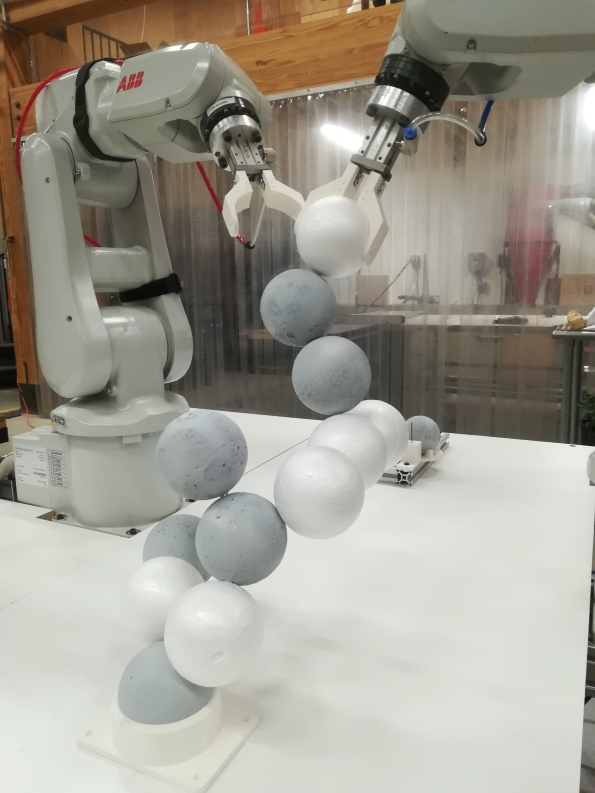
\includegraphics[trim={0cm 0cm 0cm 0cm}, clip, width=.99\textwidth]{stochastic1}
        \end{subfigure}
        %
        \begin{subfigure}{.49\textwidth}
            \centering
            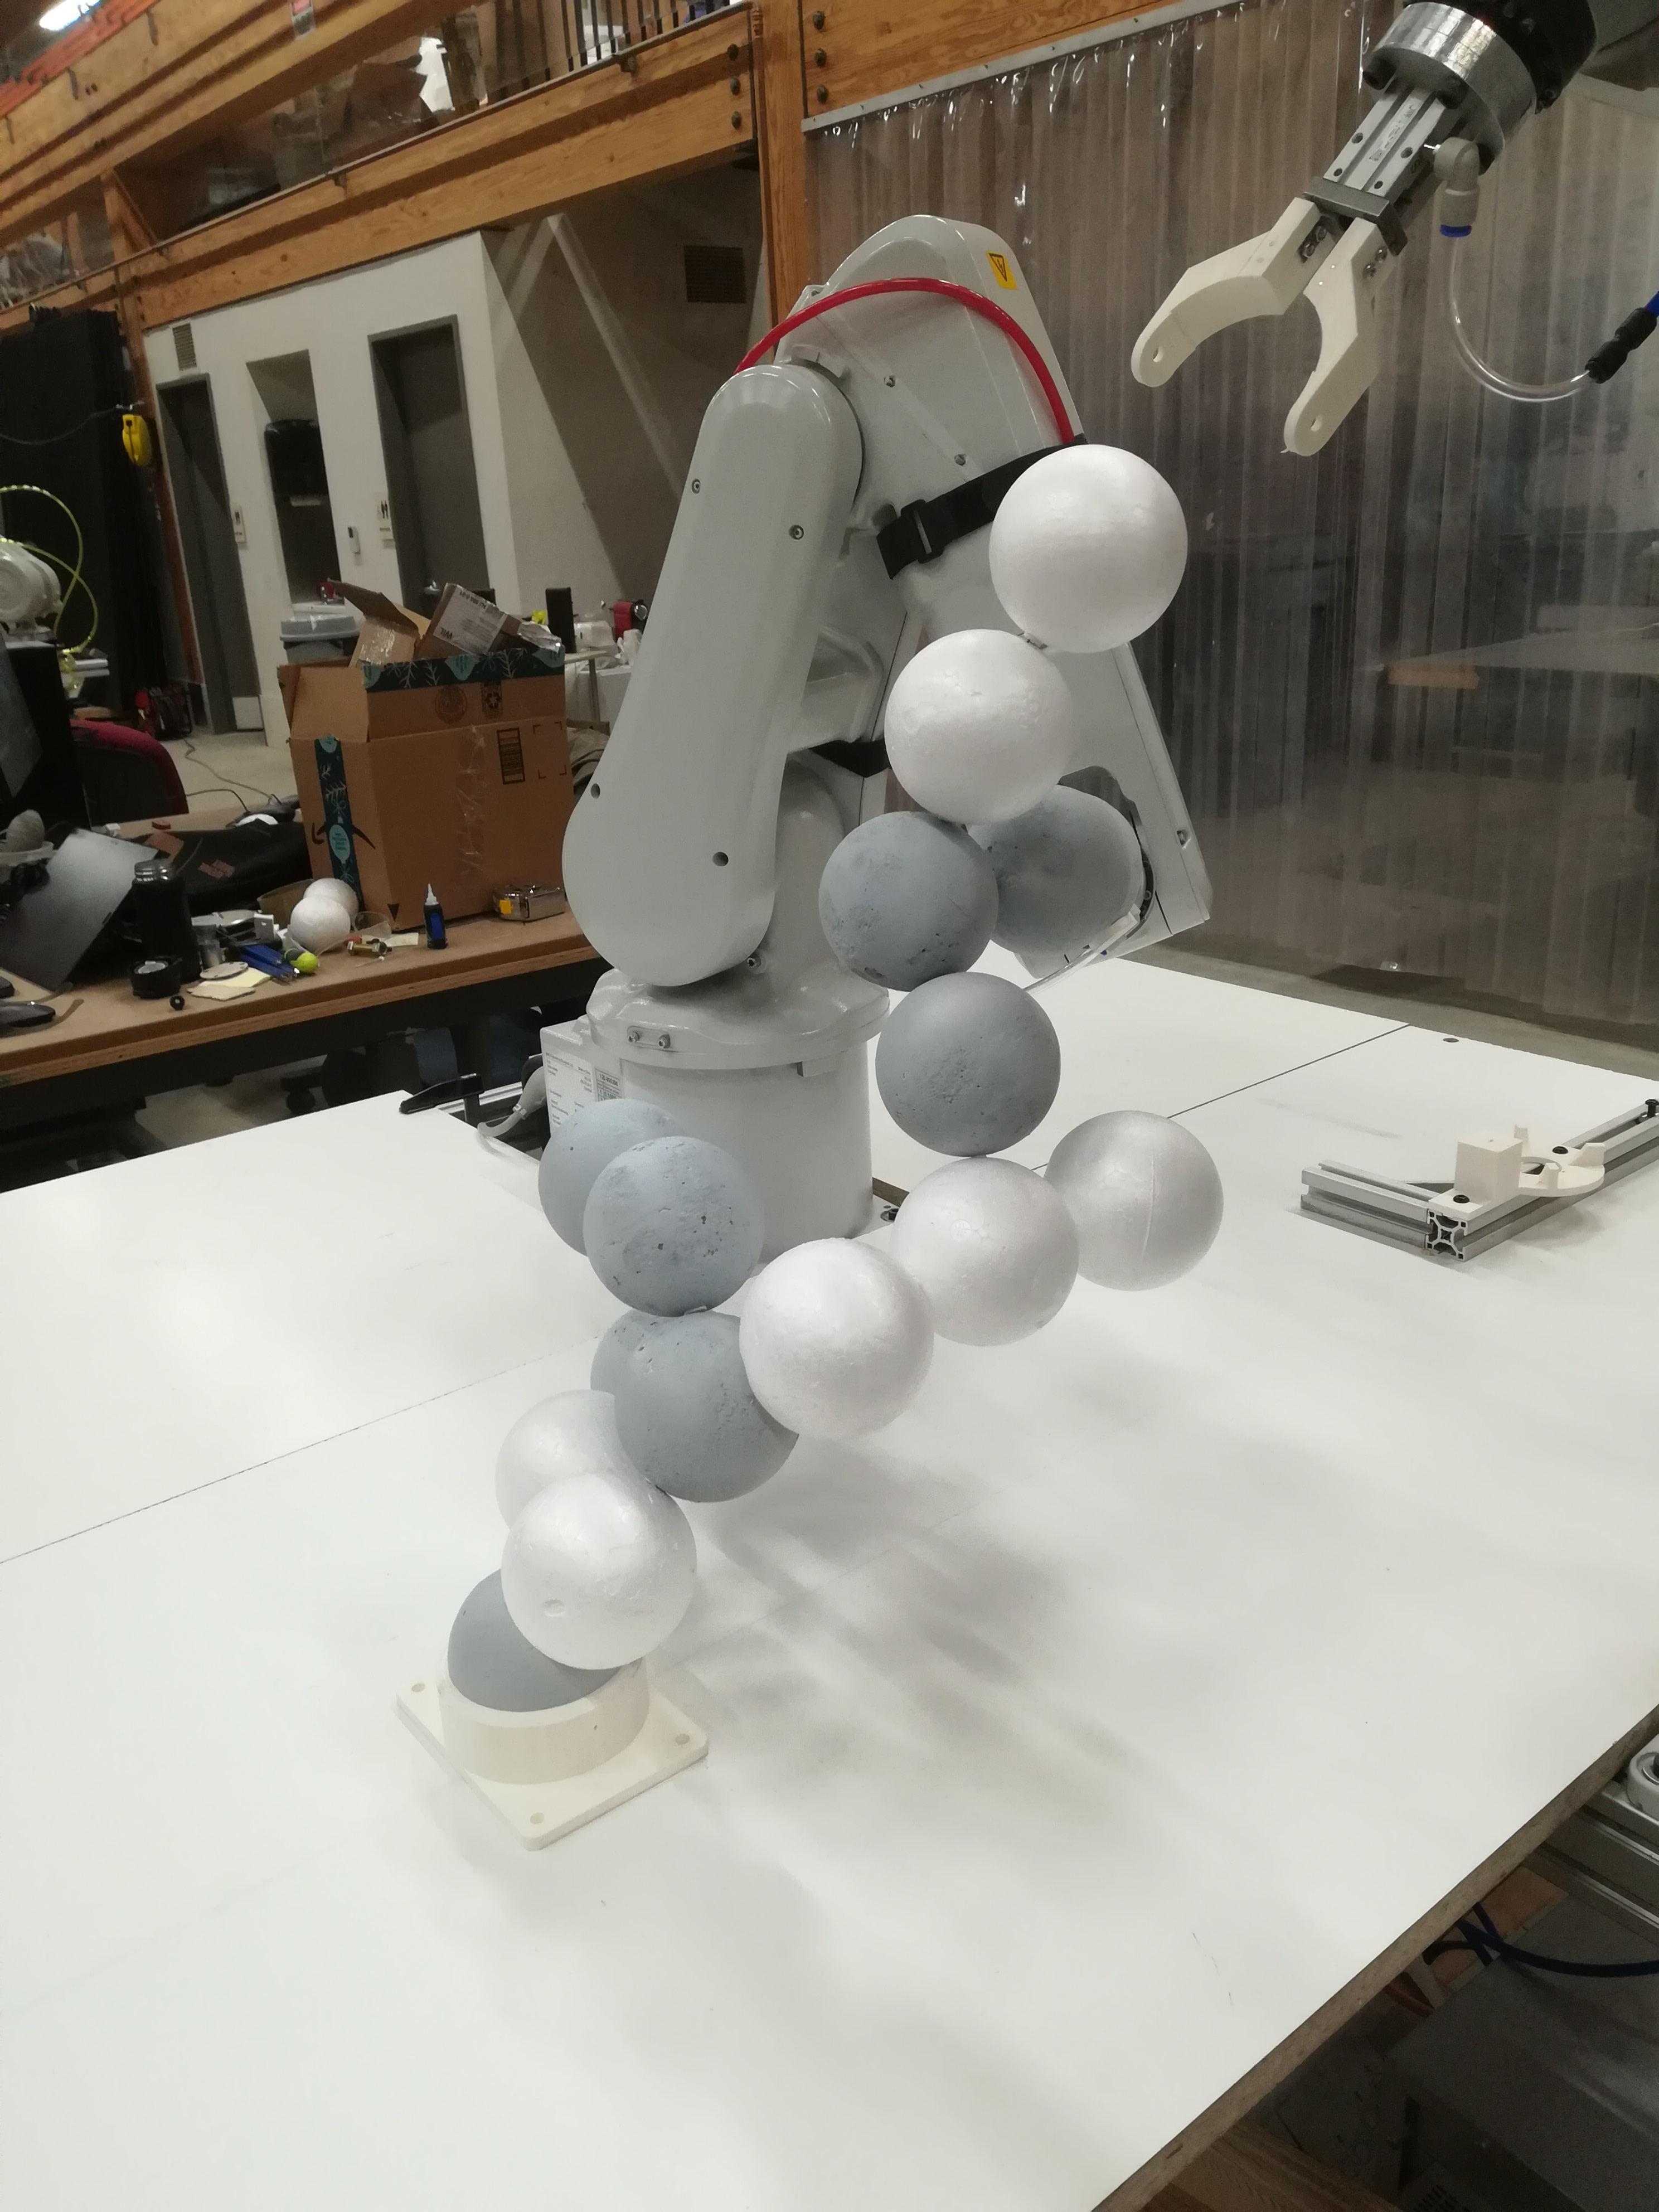
\includegraphics[trim={0cm 0cm 0cm 0cm}, clip, width=.99\textwidth]{stochastic2}
        \end{subfigure}
        \caption{Snapshots from the cooperative robotic fabrication of an unplanned structure}
        \label{fig:stochastic}
    \end{figure}  

    This project revealed the versatility of robotic arms beyond active fabrication tasks, showcasing their ability to serve as passive supports during the fabrication process. Consequently, the need for external supporting structures during fabrication was eliminated addressing the goal of material reduction as per the ``slow'' circular economy principle. Although the scale and complexity of the structure assembled in this research project was modest, its significance lies in laying the groundwork for subsequent, more complex robotic fabrication tasks and developing an interactive design strategy that involves both humans and robots.

\subsection{Cooperative Robotic Support-Place Sequencing for Scaffold-free Construction of Spanning Masonry Structures}\label{sec:04_examples_LV}
    \Cref{chap:4_LightVault} described the cooperative robotic sequencing and simulation studies as part of the LightVault project. In this project, a $3.6 \times 6.5 \times 2.2m$ doubly-curved masonry vault was built with two stationary robotic arms as a demonstration of CRF applied to an assembly process \citep{parascho_lightvault_2021}. In the first phase of the project, a central arch was constructed utilizing the alternating cooperative robotic placement and support approach inspired by previous research on the assembly of metal space frame structures \citep{parascho_cooperative_2017,parascho_computational_2018}. One robot continuously acted as a support to the partially completed arch, while the other was used to place additional bricks into the structure (\cref{fig:lightvault}). Thus, the arch was built from one end to the other without requiring any additional temporary supporting structure. The structural performance of the arch during construction was assessed using a discrete element modelling approach \citep{paris_robotic_2021}, and the cooperative sequencing was later theorised to setups with more than two robots to further improve the structural performance during assembly \citep{bruun_three_2021}. In the second phase of the project, the rest of the vault was built layer by layer using the central arch as a backbone structure \citep{parascho_robotic_2020,han_concept_2020}. 

    \begin{figure}[H]
        \centering
        \begin{subfigure}{.49\textwidth}
            \centering
            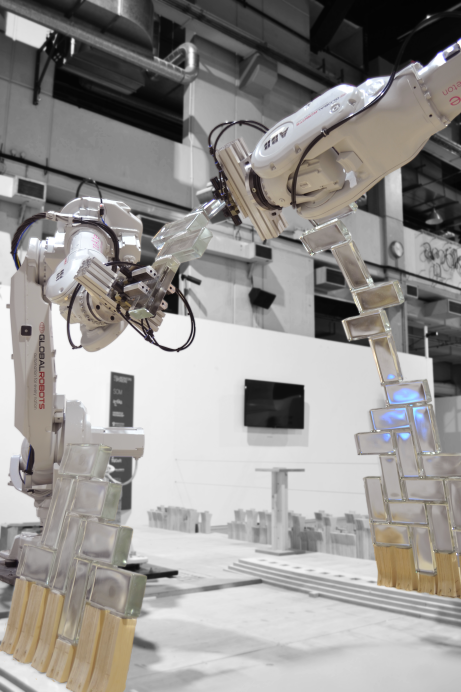
\includegraphics[trim={0cm 0cm 0cm 0cm}, clip, width=.99\textwidth]{lightvault_arch}
            \caption{first phase: backbone arch under construction}
            \label{fig:lightvault_arch}
        \end{subfigure}
        %
        \begin{subfigure}{.49\textwidth}
            \centering
            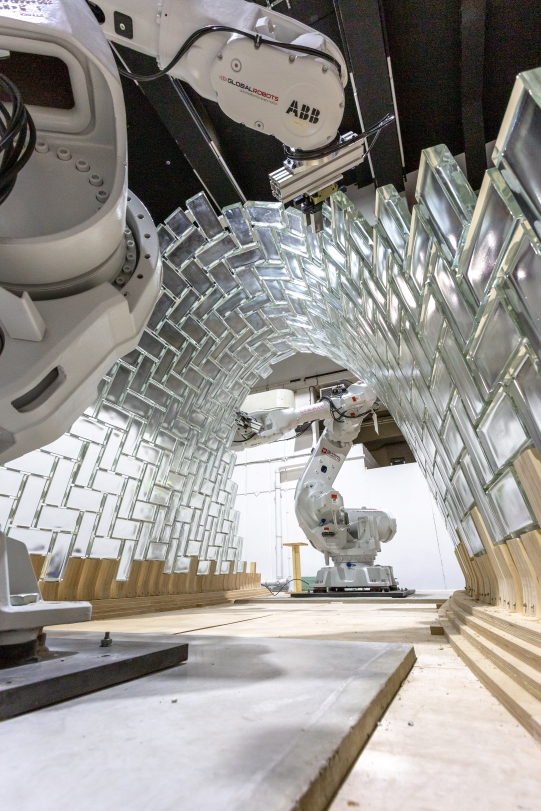
\includegraphics[trim={0cm 0cm 0cm 0cm}, clip, width=.99\textwidth]{lightvault_restofvault}
            \caption{second phase: vault under construction}
            \label{fig:lightvault_full}
        \end{subfigure}
        \caption{Scaffold-free cooperative robotic assembly of a masonry vault}
        \label{fig:lightvault}
    \end{figure}  

    Overall, this project demonstrated the first application of CRF for scaffold-free construction of spanning structures made from heavy materials (e.g., glass bricks). With respect to a circular economy, specifically the ``slow'' principle, the use of primary resources was reduced by both by eliminating temporary supporting structures and by minimizing the material necessary in the structure itself by enabling the construction of a structurally efficient but geometrically complex form that was designed to experience only compressive forces.


\subsection{Rigidity Theory for the Design of Space Frame Structures that can be (Dis)Assembled without Scaffolding}\label{sec:04_examples_frame}
    \Cref{chap:5_SpaceFrame} described the output from the Remote Robotic Assemblies workshop held at the 2021 Association for Computer Aided Design in Architecture (ACADIA) conference, where a timber space frame arch structure was first designed and then constructed using two cooperating robotic arms on linear tracks. This project was a demonstration of CRF applied to not just the assembly of the structure but extending its use for the first time to disassembly as well. Using a method based on rigidity theory, the space frame was designed explicitly to leverage cooperative robotic support sequencing to replace temporary supporting structure during both the construction and deconstruction phases \citep{bruun_structural_2022}. The structure was first assembled element by element, where one passive robotic agent was always required to provide support to the partially assembled structure. Following this, the structure was disassembled cell by cell, taking advantage of the fact that it was designed explicitly as an assembly of locally rigid tetrahedral cells. These cells where sequentially supported, isolated, and then removed with one robot, while the other robot supported the partially disassembled structure (\cref{fig:spaceframe}). The disassembly process is an example of a collaborative-CRF (Co-CRF) process as the removal of individual elements to disconnect the rigid tetrahedral cells from the remaining structure was done in collaboration with a human.

    Overall, this project demonstrated that CRF is a viable technology to reduce primary resource inputs in the form of scaffolding during both the assembly and disassembly of spanning space frame structures. With respect to a circular economy, this addresses the ``slow'' principle. In addition, extending the application of CRF to disassembly tasks highlighted the potential of including considerations for disassembly at the outset of a design to better facilitate the reuse and recycling of building components at the end of a structure's life. This design for reversibility in a scaffold-free way addresses the ``slow'' principle as part of a circular economy.

    \begin{figure}[H]
        \centering
        \begin{subfigure}{.99\textwidth}
            \centering
            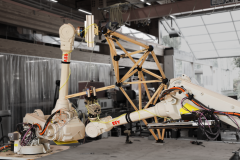
\includegraphics[trim={0cm 0cm 0cm 0cm}, clip, width=.75\textwidth]{spaceframe_place}
            \caption{Phase 1: Assembling locally rigid cells by placing one element at a time while the remaining structure is supported.}
            \label{fig:spaceframe_assembly}
        \end{subfigure}
        
        \vspace{2mm}
        
        \begin{subfigure}{.99\textwidth}
            \centering
            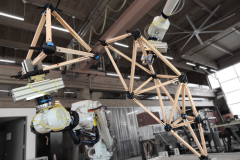
\includegraphics[trim={0cm 0cm 0cm 0cm},clip, width=.75\textwidth]{spaceframe_remove}
            \caption{Phase 2: Isolating locally rigid cells in the scaffold-free cooperative robotic disassembly of a spanning timber space frame arch structure.}
            \label{fig:spaceframe_disassembly}
        \end{subfigure}
        \caption{Scaffold-free (dis)assembly of a spanning timber space frame arch structure}
        \label{fig:spaceframe}
    \end{figure}   

\subsection{Support Hierarchy Graphs for Planning the Scaffold-Free Dis-and-Reassembly of a Frame Structure with Cooperating Robots} \label{sec:04_examples_ZW}
    \Cref{chap:6_ZeroWaste} described the development of a graph-based cooperative robotic sequdence planning approach and its physical robotic implementation as part of the ZeroWaste project. This project explored the idea of treating existing timber buildings as stores of valuable reusable material in the context of a circular economy \citep{bruun_zerowaste_2022,bruun_zerowaste_2024}. Rather than demolishing and disposing of a building at the end of its life, the goal was to leverage the use of a CRF setup to first gather data about an unknown existing structure and then use this information together with the robotic setup to disassemble and then reassemble the structure into new feasible configurations.
    
    As the starting point, a pavilion-scale timber structure was built manually to act as a stand-in representing a generic unknown existing structure built according to standard stick framing construction practices. Next, 3D cameras were mounted on two robotic arms, which were then used to take several point cloud captures of the structure from various locations and angles. Using the accurate positional information queried from the robotic controller, the individual point cloud captures were transformed and then stitched together to create a complete spatial model of the existing structure. Creating this complete model was only possible when using multiple robots, as a single robot would not have the required reach and manoeuvrability to fully capture the structure. For an existing building, the exact geometry and spatial location of the structure is not known, thus the as-built geometric information gathered in this imaging process was necessary when later planning the RF sequences.

    Next, scaffold-free robotic cooperative disassembly and reassembly sequences were calculated algorithmically using a support hierarchy graph representation of the structure. These sequences were specifically planned for execution with the three robotic arms available in the fabrication cell, two on linear tracks and one stationary, without requiring external temporary formwork. The physical RF process was split into four distinct phases, targeting different objectives with respect to the cooperative robotic sequencing and the degree of disassembly and reassembly (\cref{fig:zerowaste}). \Cref{chap:6_ZeroWaste} solely encompasses phases 1, 2, and 3, as outlined in the published research paper that is integrated into this dissertation. The final phase, while yielding an aesthetically captivating structure, was completed without the use of a cooperative robotic framework and therefore falls outside the main research scope if this dissertation.

    \begin{figure}[H]
        \centering
        \begin{subfigure}{.49\textwidth}
            \centering
            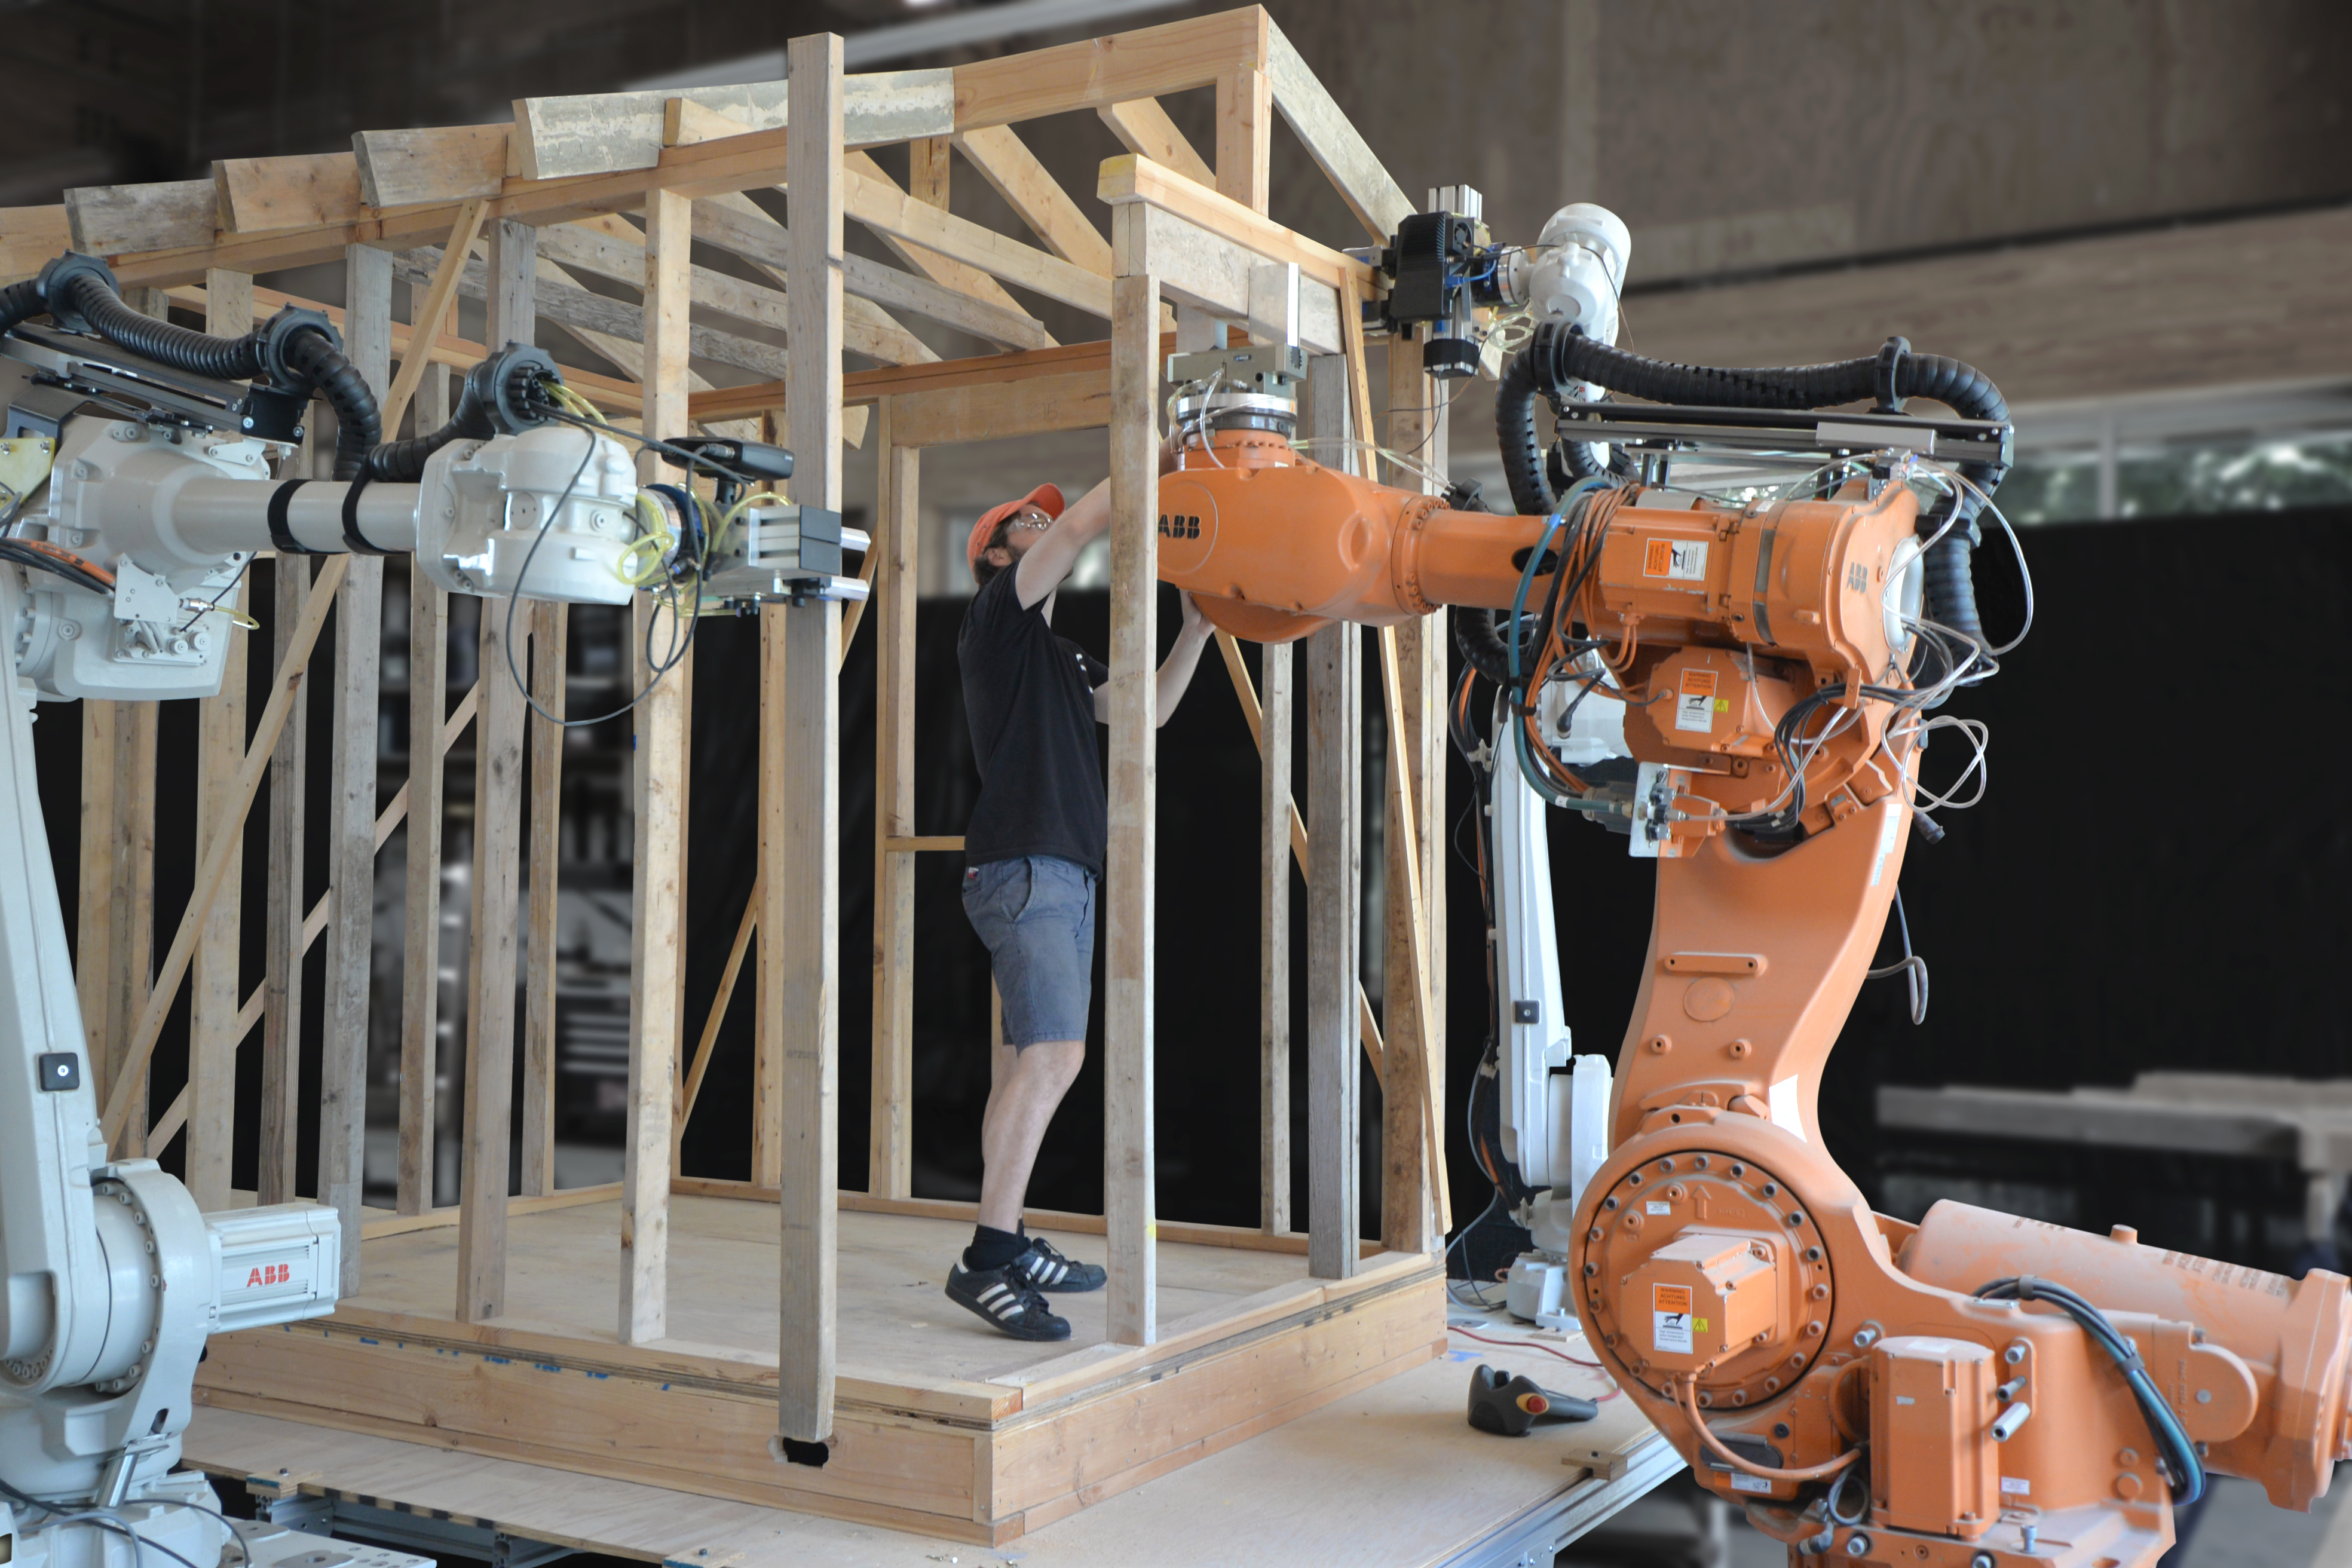
\includegraphics[trim={0cm 0cm 0cm 0cm}, clip, width=.99\textwidth]{zerowaste_p1}
            \caption{phase 1}
        \end{subfigure}
        %
        \begin{subfigure}{.49\textwidth}
            \centering
            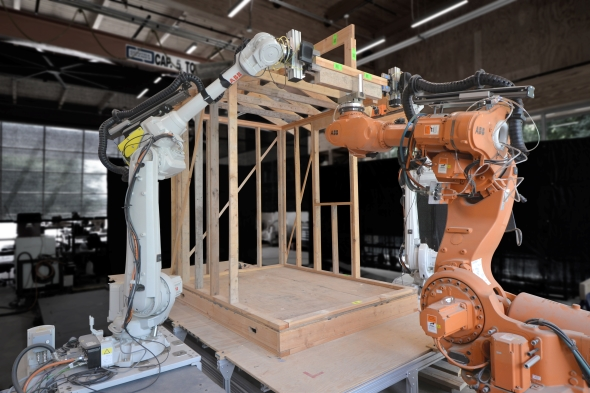
\includegraphics[trim={0cm 0cm 0cm 0cm}, clip, width=.99\textwidth]{zerowaste_p2}
            \caption{phase 2}
        \end{subfigure}

        \begin{subfigure}{.49\textwidth}
            \centering
            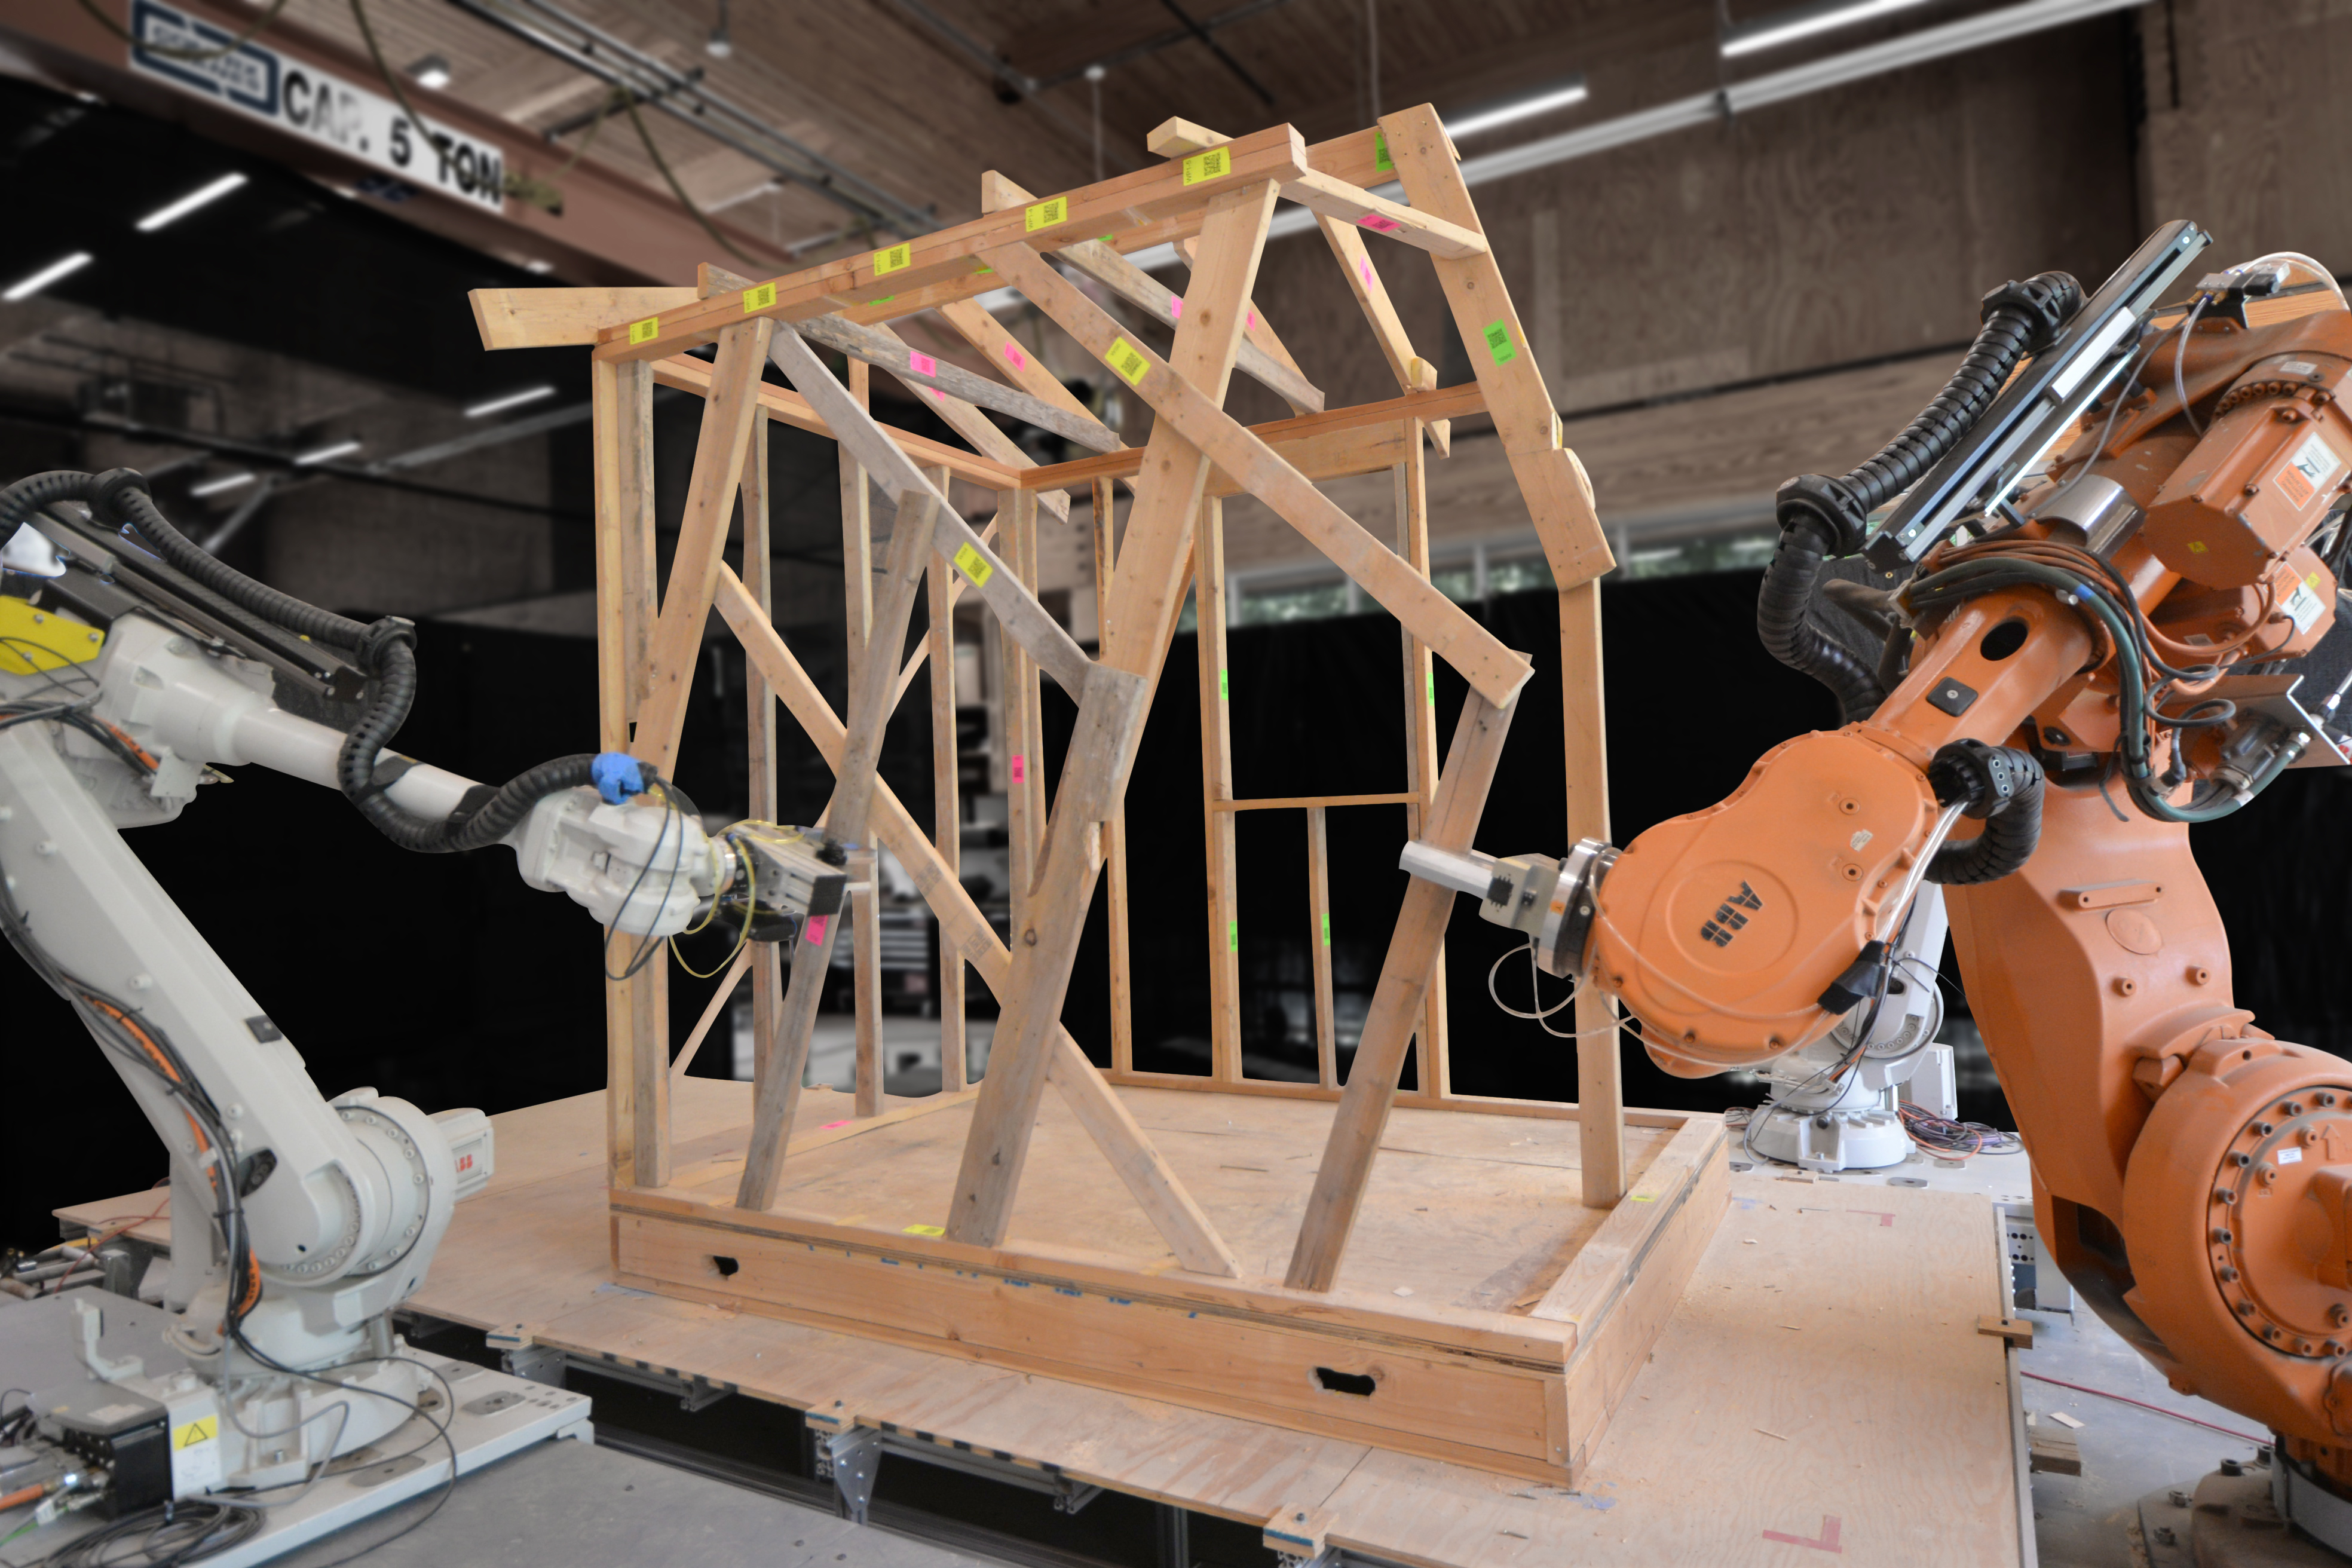
\includegraphics[trim={0cm 0cm 0cm 0cm}, clip, width=.99\textwidth]{zerowaste_p3}
            \caption{phase 3}
        \end{subfigure}
        %
        \begin{subfigure}{.49\textwidth}
            \centering
            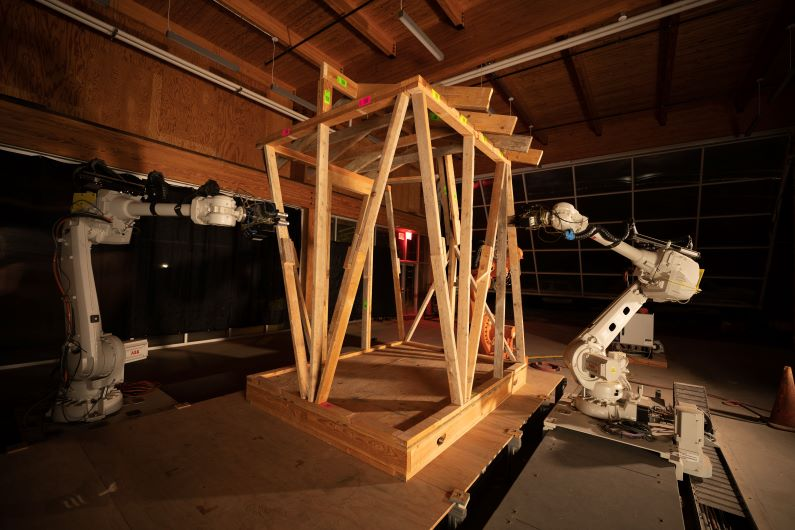
\includegraphics[trim={0cm 0cm 0cm 0cm}, clip, width=.99\textwidth]{zerowaste_p4}
            \caption{final structure}
        \end{subfigure}
        \caption{Snapshots from the different phases of the cooperative robotic disassembly and reassembly as part of the ZeroWaste project}
        \label{fig:zerowaste}
    \end{figure}   

    Similarly to the project described in \cref{sec:04_examples_frame}, ZeroWaste demonstrated the use of a CRF setup in providing temporary support to a structure during disassembly, but further extended its use to perform scaffold-free reassembly and reuse of removed material. Improvements in construction efficiency were also demonstrated as the full fabrication process only required a single person working alongside the robots, whereas using non-robotic methods would typically require several workers to accomplish the same tasks. Overall, the successful use of CRF in the ZeroWaste project to assist in structural disassembly and reassembly tasks highlighted the potential of this technology to facilitate a more circular treatment of existing timber building stock through its reuse.


% ----------------------------------------------------------------------------------------------------
% Bibliography
% ---------------------------------------------------------------------------------------------------- 
\section{Recommendations for Future Research} \label{sec:03_04_future}
    The four robotic fabrication research projects outlined in this dissertation mark a significant advancement in showcasing innovative applications of scaffold-free cooperative robotic disassembly and reassembly processes for discrete element structures. At the same time, their completion also highlights several promising avenues for future research. While each chapter delves into project-specific limitations and potential research endeavors, this section aims to consolidate these discussions into broader categories that are broadly applicable across the research presented in the whole dissertation. Pursuing these future research directions promises to further improve the capabilities of cooperative robotic fabrication systems in the construction industry, thereby fostering more sustainable and efficient construction practices.

    \subsection{Human-Robot Collaboration}
        The research presented in this dissertation is primarily focused on cooperative robotic processes, wherein multiple robots collaborate to tackle tasks beyond the abilities of a single robot. While these processes exhibit remarkable potential, incorporating humans into the design and fabrication loop could significantly augment the utility and effectiveness of the overall setup. Despite various degrees of human involvement in realizing all the robotic fabrication demonstrator structures, such as material preparation, code execution, fabrication sequence planning, and data processing, only the research presented in \Cref{chap:3_humanrobot} showcased genuine human collaboration within a collaborative-cooperative robotic fabrication process, albeit at a limited structural scale.

        Future research endeavors should center on refining fabrication processes to facilitate both cooperative sequencing among multiple robots while accounting for more direct human involvement in both the design and fabrication phases. This approach promises to unlock new avenues for digital and human collaboration, thereby fully harnessing the capabilities of robotic manipulators as indispensable design-fabrication tools. However, such collaboration between humans and robots requires further investigation into how to create a safe environment and workflow that would allow for both human-robot and robot-robot interactions to occur seamlessly.

    \subsection{Real-Time Control Through an Augmented/Virtual Reality Environment}
        One notable limitation across all fabrication projects in this dissertation is the absence of real-time operation. In other words, users had to pre-plan fabrication processes, including robot sequencing and path planning, leading to a significant delay between planning and execution of fabrication tasks. While this approach is valid in many scenarios, it inherently introduces a time lag that can be prohibitive with respect to construction efficiency.

        Future research should prioritize implementing cooperative robotic sequencing and control in a real-time environment. This could be achieved through autonomous robotic processes, where decisions regarding motion and execution are made based on predefined criteria, adapting in real-time to the evolving environment. Alternatively, a control method akin to current robotic usage could be employed just in a more efficient manner. Rather than users performing multiple offline steps before instructing the robots by executing blocks of code on a teach pendant, they could have direct connectivity to the robots and control them through wearable sensors.
        
        For instance, users could wear augmented/virtual reality goggles coupled with gloves with motion capture targets. Through augmented/virtual reality, users could perceive the robot's work environment and manipulate objects using hand gestures, with the sensors on the gloves corresponding to the robot's motion. This approach allows users to execute simple actions ergonomically, translating digital manipulations into physical robot actions.
        
        Moreover, this real-time control method could facilitate remote operation, eliminating the need for users and robots to be physically co-located. As long as the augmented reality environment mirrors the robot's operating space and there's a wireless link between the user's arm motion and the robot's action, remote operation becomes feasible.
    
    \subsection{Mixed Fixed/Mobile Robot Teams}
        This research presented in this dissertation primarily focused on cooperative robotic fabrication within controlled laboratory settings. The robots utilized are typically fixed to the ground or operate on linear tracks. However, this approach encounters scalability issues, as the number of these larger fixed robots capable of operating simultaneously in a confined space is restricted. Although fixed or linearly mobile robotic arms can be deployed on-site, as demonstrated in the LightVault project, their calibration and accuracy present significant challenges in active job site environments.

        Nonetheless, this does not negate the potential role of such robotic setups on-site; rather, it underscores the necessity of enhancing flexibility by integrating mobile robots into the cooperative team. Future research should aim to broaden the field of cooperative robotic fabrication to incorporate mobile robots working alongside fixed robots. Despite mobile robots often having smaller payloads than fixed ones, their extended range, flexibility, and improved dexterity compensate for this limitation.

        Therefore, a more resilient and adaptable robotic setup would integrate both fixed and mobile robots, possibly including human interaction as well. Each agent would undertake tasks suited to its capabilities. For instance, mobile robots could excel in tasks like data gathering and light material handling, while larger robots could handle long-duration tasks such as structural support, thereby enhancing the setup's overall flexibility and range of applications.

        Integrating mobile robots with stationary robotic arms would streamline labor distribution and expand the setup's capabilities to manage larger and more varied construction scenarios. Moreover, mobile robots could supplant manual execution of tasks requiring fine motor skills typically performed by humans, such as fastener manipulation, thereby enhancing efficiency, precision, and the level of automation in the fabrication process.

    \subsection{Incorporating Sensor Feedback in Design Process}
        Future research will integrate feedback mechanisms, such as real-time 3D imaging of the structure during assembly or disassembly, to enhance the adaptability of the fabrication process to changing conditions, such as structural deformation due to self-weight. This approach will enable the fabrication process to directly adjust to unpredictable changes or deformations as they occur.

        For example, in the ZeroWaste project, a current limitation arises from relying on pre-scanning the structure to generate a point cloud before initiating fabrication planning. However, the method lacks the ability to promptly and accurately update the point cloud model with changes during fabrication, necessitating a complete re-scan for significant updates. Future research should prioritize developing processes that allow robots to dynamically collect information and update the as-built point cloud model while simultaneously performing fabrication tasks. This real-time feedback mechanism would enhance adaptability and accuracy in planning and executing fabrication processes, especially for complex and dynamically changing structures.

        Additionally, employing a force-torque sensor mounted on the robot gripper could inform the placement of new components in locations that minimize total unbalanced force. These force-torque sensors, mounted on the robot tool flange, could also facilitate cooperative in situ non-destructive testing on structures, providing valuable data on their performance during assembly or disassembly, such as determining stiffness. This data can be used to design more material-efficient structures, assess overall structural performance during fabrication, and measure parameters like stiffness or degree of damage to a member. Each robot could effectively act as a 6-degree-of-freedom actuator capable of applying forces and moments to the structure at any location and orientation in space. By sequencing robots cooperatively, it becomes feasible to apply non-standard loading conditions, which would be challenging to evaluate in situ using conventional load testing methods, particularly for geometrically complex structures.

    \subsection{Path Planning and Structural Analysis Integration}
        Another area for future research involves simplifying the manual steps needed to set up and process the results of path-planning and reachability feasibility assessments. Currently, users must manually select multiple locations in the digital environment representing the structure and robotic system to conduct a series of brute force path-planning and reachability checks at these locations. This preparation process is time-consuming and labor-intensive. Future research should explore automated methods for this process, potentially utilizing machine learning and computer vision techniques to automate point cloud processing for path-planning checks.

        Similarly, implementing a more automated approach to creating the finite element model for assessing the progressive behavior of the structure during a robotic process would speed up structural feasibility assessments. For example, in the ZeroWaste project, users manually process the point cloud to construct the structural analysis model for each sequence, based on the centerline locations of members.

        Enhanced integration between structural results from finite element analysis and the robotic path planning process would enable the creation of a more informed optimization process for generating and selecting fabrication sequences. Establishing an automated workflow to select a fabrication sequence based on optimization criteria linked to structural performance during fabrication would lead to a faster and less manual sequence generation process across all the different applications described in this dissertation. For instance, if relying on a graph-based method, the could be formulated as an optimization problem by setting edge weights in the graph based on the structural loading or other structural criteria of interest. Then, the objective function for the problem could be formulated to minimize the cumulative value across the graph representing the structure during the entire fabrication process. Overall, better integration of finite element structural results, the robotic path planning process, and a graph representation used to suggest feasible robotic sequences would reduce the manual work required for planning a cooperative robotic fabrication process.

    \subsection{Applications to Continuous Material Systems}
        The research chapters in this dissertation focused on the robotic fabrication of discrete element structural systems, such as space frames, masonry structures, and stick frame structures. Moving forward, research should explore employing cooperative robotic techniques for continuous material systems.

        For instance, in 3D printing of concrete, current methods typically utilize a single robot or print-head to extrude material layer by layer, limiting the ability to create complex shapes with inclined or sloping geometry. An avenue for future exploration involves employing cooperative robotic methods to enable the construction of more intricate shapes. One approach could involve one robot performing the printing while another provides temporary support to inclined or sloping concrete layers. Additionally, the supporting robot could handle tasks like placing reinforcement bars or other structural elements within the 3D printed concrete structure, tasks that are currently either manual or not performed at all.

        Another potential application lies in metallic additive manufacturing or continuous welding processes. In this scenario, one robot would handle material placement while the other would perform inspection and monitoring of the material deposition. This setup enables real-time correction or adjustment of the process, ensuring quality and precision throughout fabrication.

    \subsection{Increased Payload and Work Area}
        One limitation of the research presented in this dissertation stems from the inherent physical constraints of the available robotic setup. While having access to three larger-scale robotic arms presents a unique opportunity for innovative research, certain limitations affect the scope of exploration. Specifically, two of the robots were confined to a linear travel of 3.9m on tracks spaced 3.45m apart, defining the reachable work area. Additionally, the third robot was fixed to the ground without a track, further restricting its reach and motion capabilities.

        Ground-mounted robots inherently face limitations in their reach, especially in height, thereby constraining the cooperative build volume to a small area between the two tracked robots. This spatial restriction is depicted in \Cref{fig:ecl_setup}, illustrating the limited cooperative reach zone formed by the two robots.

        \begin{figure}[h]
            \centering
            \begin{subfigure}{.49\textwidth}
                \centering
                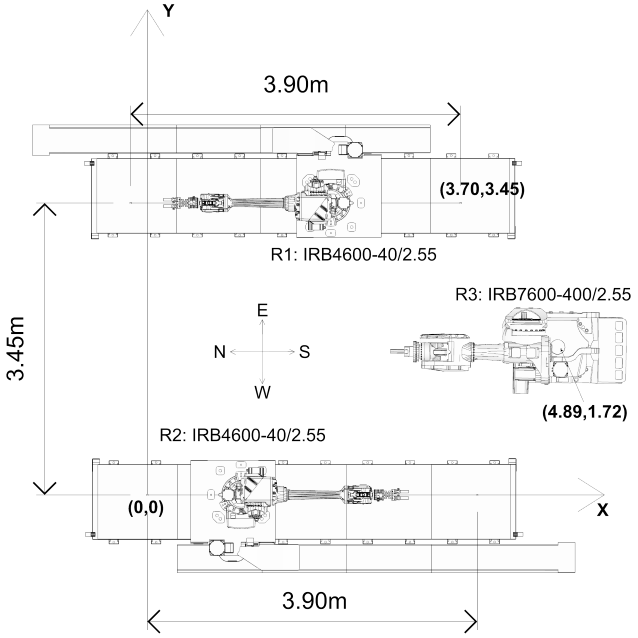
\includegraphics[trim={0cm 0cm 0cm 0cm}, clip, width=.99\textwidth]{ecl_robot1}
                \caption{Plan view of robotic cell}
            \end{subfigure}
            %
            \begin{subfigure}{.49\textwidth}
                \centering
                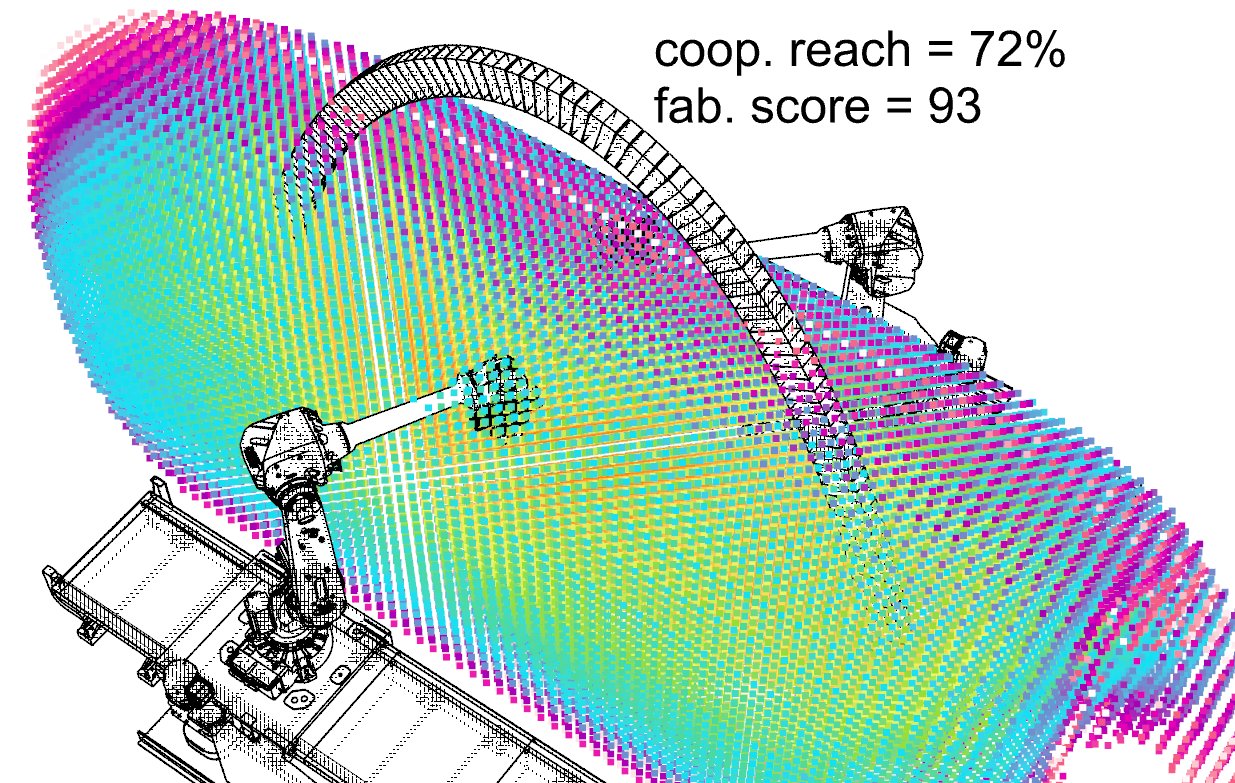
\includegraphics[trim={0cm 0cm 0cm 0cm},clip, width=.99\textwidth]{ecl_robot2}
                \caption{Limited volume where both track robots could reach}
            \end{subfigure}
            \caption{Robotic setup used throughout dissertation research}
            \label{fig:ecl_setup}
        \end{figure}   

        \newpage
        Moreover, the payload capacities of the robots serve as another limiting factor, impacting the size and scale of structural components that can be manipulated and supported during construction. While the two tracked robots had a payload limit of 40kg each, sufficient for handling lighter materials and tasks at reasonable scales, this limit remained a significant constraint. The third fixed robot had a payload capacity of 400kg; however, due to its limited reach without a track, it primarily served support functions and some restricted material handling tasks.

        To address the physical limitations affecting the type and size of structures that can be constructed and disassembled robotically, future efforts should concentrate on establishing a more adaptable and versatile laboratory environment. 

        \Cref{fig:gt_setup} depicts a novel research facility developed by the author for future research that features an overhead cartesian gantry system supporting two suspended robots, along with a heavy-payload robot mounted on a track. This setup is inspired by the Robotic Fabrication Lab (RFL) for the Institute of Technology in Architecture (ITA) on the Hoenggerberg Campus of ETH Zurich \cite{chair_of_architecture_and_digital_fabrication_robotic_2016}. By suspending two robots from an overhead gantry capable of movement in the X, Y, and Z axes, complete reachability across a significantly larger work volume is achieved, resolving the previous issue of limited cooperative work zones. For the purpose of scale comparisons, the current robotic research setup utilized to construct the physical demonstrators described in this dissertation is shown inside the gantry work area. 

        The gantry provides a spacious working area measuring approximately 16.6 by 6.7 meters, with a height clearance of up to 4.2 meters. Furthermore, the suspended robots on the gantry's Z-axis boast significantly higher payload capacities compared to robots mounted on tracks in the current setup used by the author of this disseration in the course of their research. With a payload capacity of 200kg each, these suspended robots can accommodate larger tools and manipulate more substantial structural elements, facilitating the completion of more intricate fabrication tasks.

        \begin{figure}[H]
            \centering
            \begin{subfigure}{.99\textwidth}
                \centering
                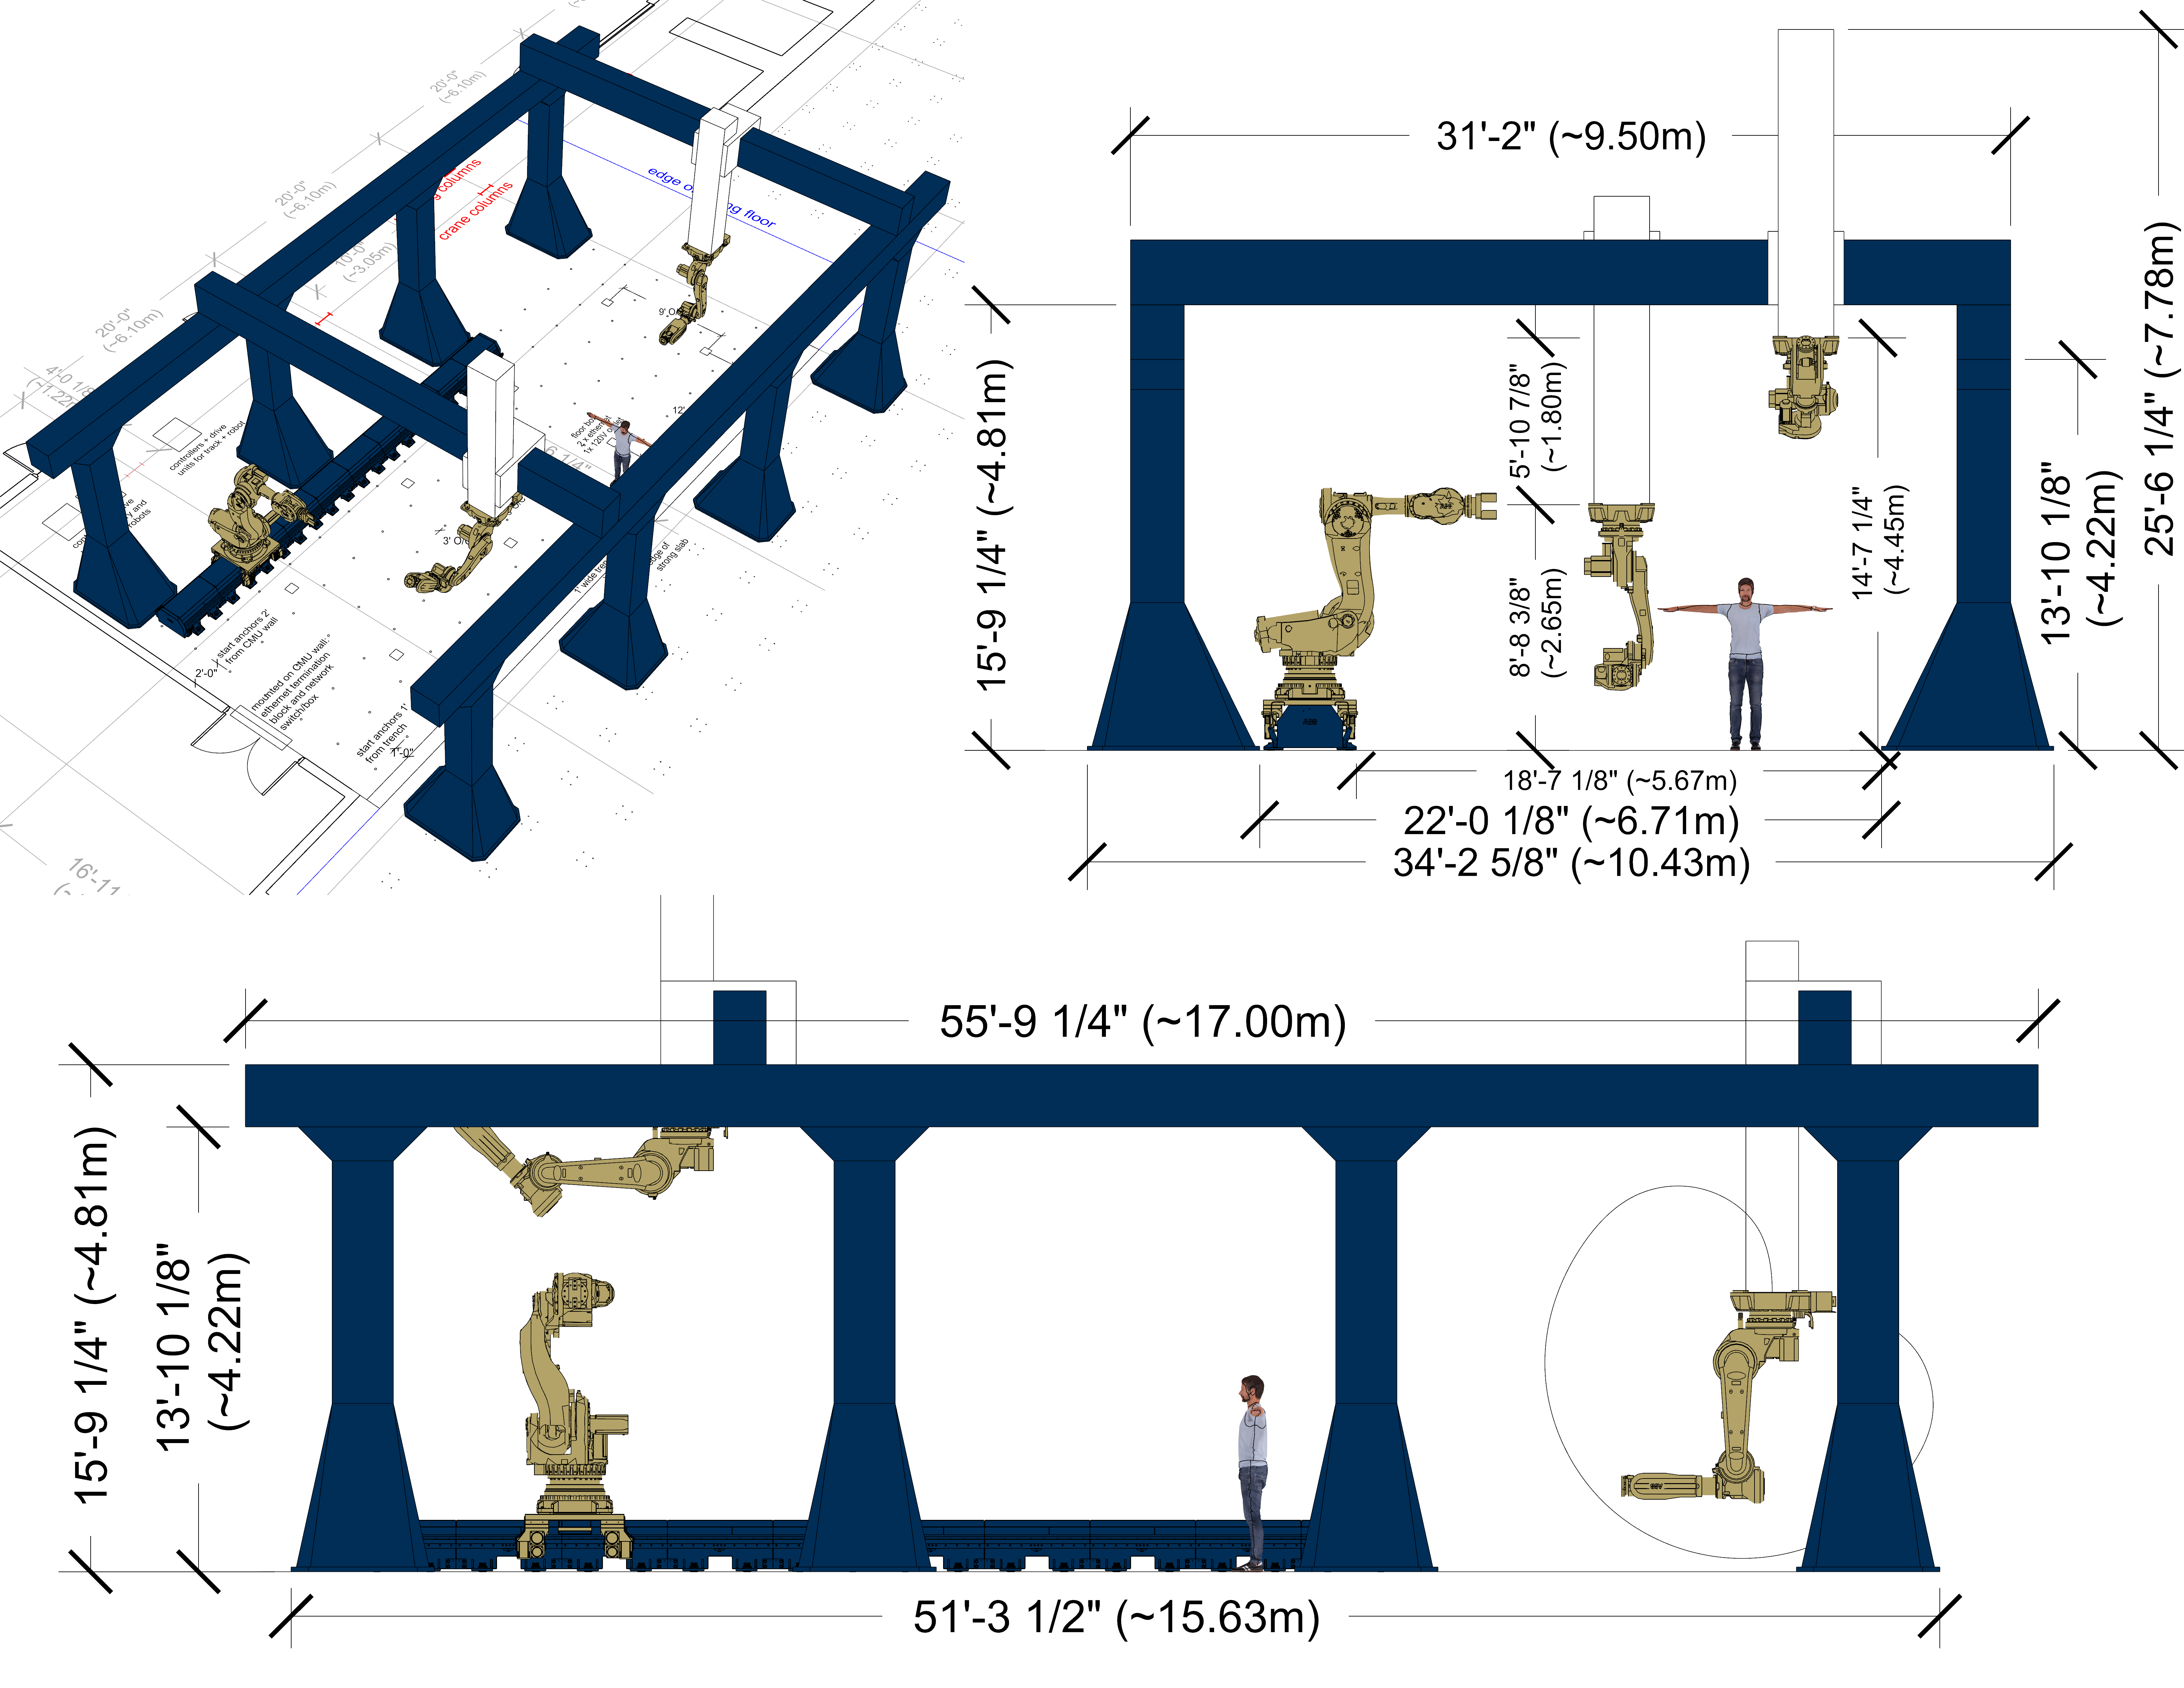
\includegraphics[trim={0cm 0cm 0cm 0cm}, clip, width=.80\textwidth]{gt_gantry1}
                \caption{various views of the robotic gantry setup}
            \end{subfigure}
            %
            
            \begin{subfigure}{.99\textwidth}
                \centering
                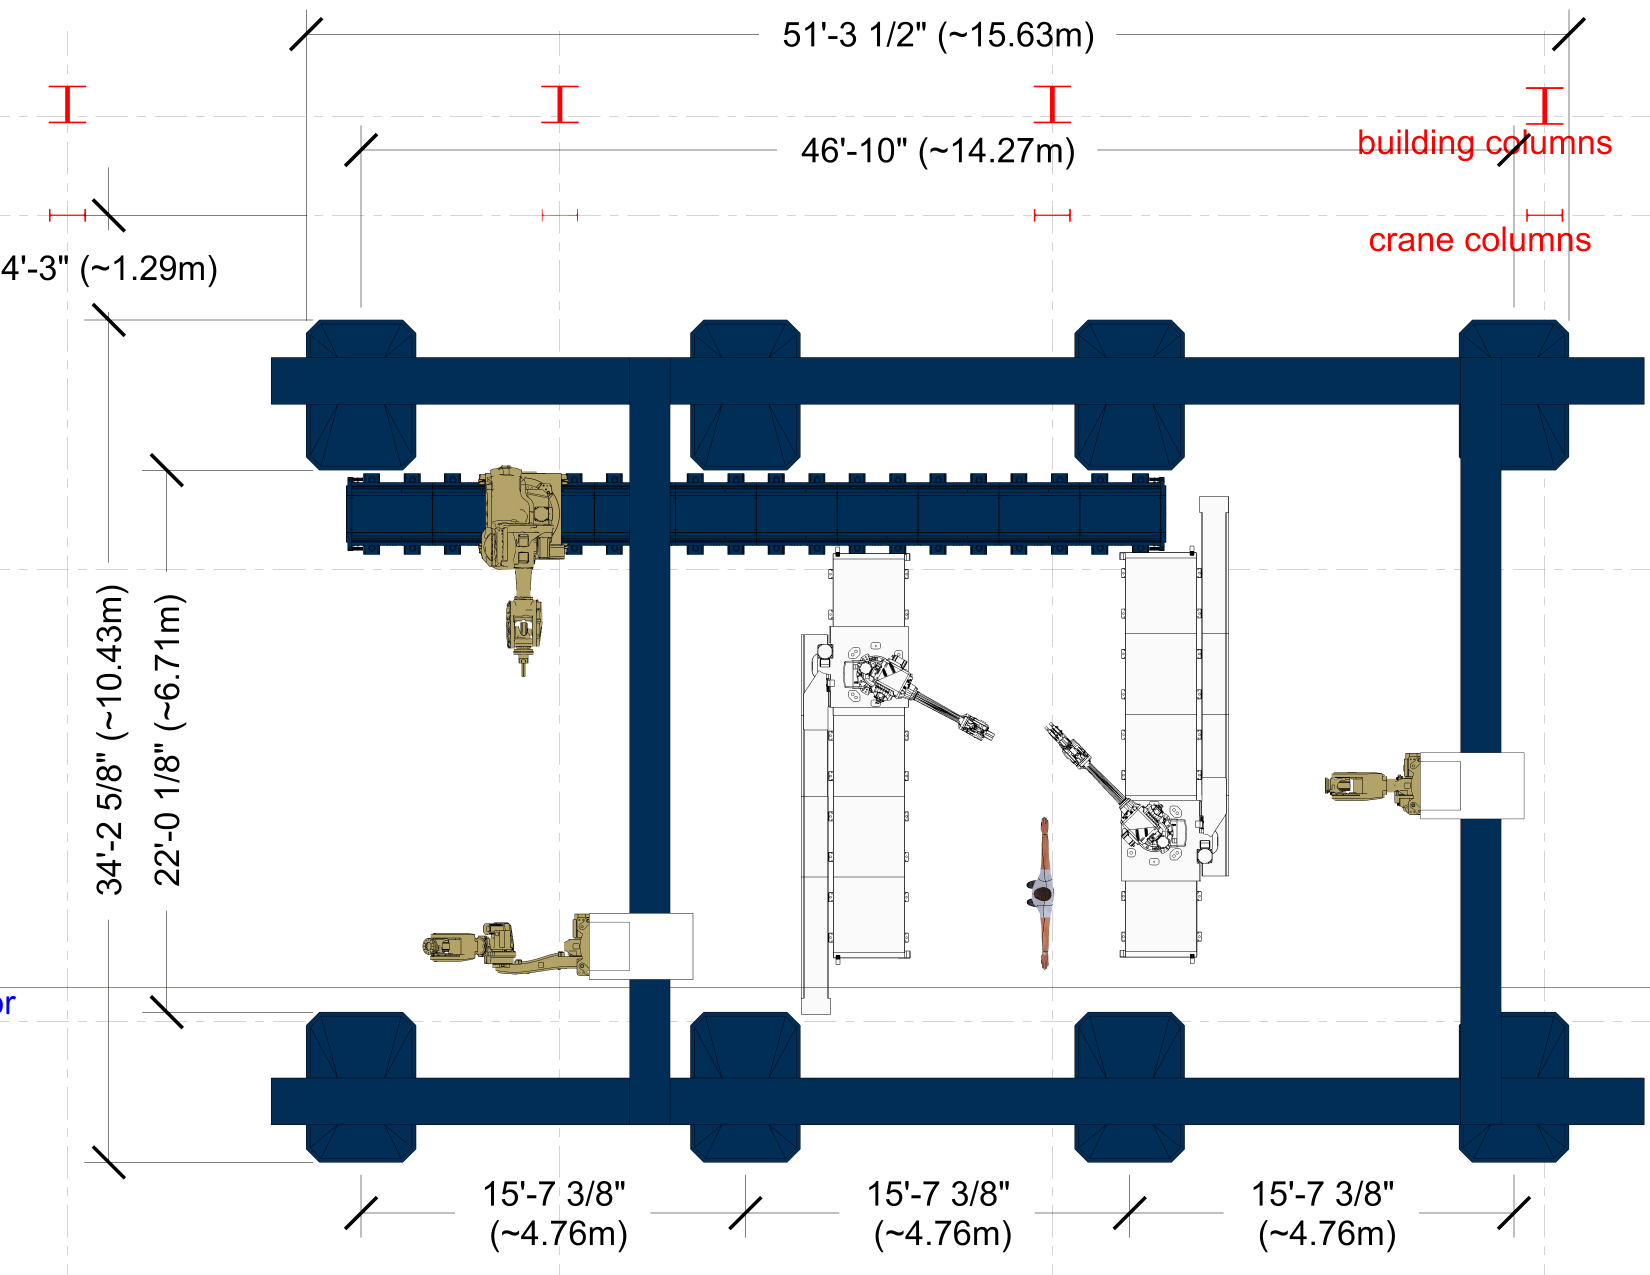
\includegraphics[trim={0cm 0cm 0cm 0cm},clip, width=.80\textwidth]{gt_gantry2}
                \caption{plan view of the gantry setup with the Princeton ECL setup in the middle for scale}
            \end{subfigure}
            \caption{Conceptual cooperative robotic gantry setup improving payload and reach.}
            \label{fig:gt_setup}
        \end{figure}   

    \section{General Conclusion}
        The global population is on a trajectory of rapid growth, with estimates projecting a population of 9.8 billion by 2050. This growth, accompanied by accelerating urbanization, emphasizes the urgent need for the architecture, engineering, and construction (AEC) industries to innovate and develop new technologies. These innovations are crucial for meeting the escalating infrastructure demands while simultaneously addressing the significant environmental impacts that stem from high energy consumption and CO2 emissions. Robotic automation in the AEC industry has the potential to enable novel construction processes for geometrically complex structures. The research presented in this dissertation demonstrates the use of Cooperative Robotic Fabrication (CRF) setups, where multiple robots collaborate on construction tasks, for applications in the assembly, disassembly, and reuse of discrete element structures, developing and showcasing computational methods that coordinate multiple robotic arms to ensure structural stability without the need for external supports or scaffolding.
        
        The dissertation begins with CRF applications focused solely on assembly and then extends to more complex tasks that involve structural disassembly and reuse. It introduces a bottom-up human-robot design framework where two cooperating robots aid in designing branching spatial structures in pseudo real-time, incorporating path-planning constraints in conjunction with human decision-making. Following this, the research showcases CRF for constructing geometrically intricate spanning masonry structures. In these scenarios, the structure is modeled as a lumped spring system, and robots are sequenced in a manner that ensures the stability of the central arch without external scaffolding. Next, the dissertation  demonstrates a fabrication-informed approach for designing space frame structures, using rigidity theory and Henneberg planar graph assembly steps to build rigid space frames intended for scaffold-free assembly and disassembly. Finally, CRF is applied to the disassembly and reuse of an existing prototype structure, satisfying circular economy principles by minimizing material waste and facilitating reuse. This is achieved through a novel graph-based method that uses the concept of structural support hierarchy to isolate affected members within the structure and generate sequences for removing these members without destabilizing the remaining structure.
        
        The research presented in this dissertation does not claim to solve all the challenges currently facing the AEC industry. However, it provides a crucial step forward in promoting the adoption of novel automation techniques and technologies. Specifically, this dissertation illustrates how structures can be designed to leverage advanced robotic assembly and disassembly techniques more effectively. The research demonstrates the potential of multiple robots working cooperatively to enhance the construction of discrete element structures such as masonry vaults, space frames and timber structures. This cooperative multi-robotic approach can significantly reduce or eliminate the need for scaffolding and temporary supports during both assembly and disassembly phases, thus minimizing overall material usage and waste.

        While this dissertation highlights the potential of robotic arms to transform construction processes, future work will aim to adapt the computational methods and cooperative robot sequencing developed here to a broader array of applications and structural typologies. Notably, the groundwork for this adaptation is already being laid, as the methods proposed in this dissertation are designed to be easily applied to other systems. This is an important contribution to the field.
        
        Limitations due to small work volumes and payloads of the robotic setup for cooperative robotic processes were also a significant constraint experienced in all of the research conducted as part of this dissertation. Thus, for further innovation in the structural cooperative robotic research space to occur, larger and more flexible research apparatuses, such as a gantry and suspended robot setup with increased reach and payload, will be necessary at the institutional level. By continuing to innovate in automation technology, the AEC industry can progress towards more sustainable and efficient construction practices. These practices are essential to meeting the demands of a growing and urbanizing global population while continuously striving to limit their environmental impact.
        
% ----------------------------------------------------------------------------------------------------
% Bibliography
% ----------------------------------------------------------------------------------------------------  
\newpage
\bibliographystyle{\BiblioPath/elsarticle-num} 

\begingroup
    \hypersetup{hidelinks}
    \bibliography{\BiblioPath/2ResearchContext}
\endgroup